\chapter{Introduction}
\label{cha1}
\chaptermark{Introduction}

Traditional images contain informations of colors of some scenes, and when stored as typical image formats in computers, these images usually are converted to some specific color spaces for the convenience of displayers, for example, jpeg format use s-RGB space. This interpretation of images provides the fundamental of most image processing tasks and their solutions, from simple tasks such as edge detection, to difficult tasks such as scene understanding.

With the development of technologies, for present days it is possible to get more informations other than merely color. In this thesis we will mainly focus on depth informations, which will be referred to as \emph{depth map}. \emph{Depth maps} are images containing information relating to the distance of the surfaces of scene objects from a viewpoint. The depth information directly provides the clue for the spacial relation of the objects in some scene, which is vital in many image processing problems, such as semantic segmentation and object recognition. At the same time, the usage of depth map introduces new tasks: the acquisition of high quality depth map, the registration of corresponding depth map and color images, etc. 

In this thesis we will study the both sides of the utilization of depth maps: in chapter~\ref{cha2}, we propose a local-linear fitting based depth upsampling algorithm to obtain high resolution and accurate depth map, as well as overcoming the intrinsic missing points problem; and in chapter~\ref{cha3}, we exploit the depth map to construct a synthesized outdoor scene dataset obeying the atmospheric model, for the benchmarking of image dehazing algorithms.

This chapter is organized as follow: section~\ref{sec:1.1.depthmap} provides the background on the acquisition and defects of depth maps; section~\ref{sec:1.2.dehaze} discusses the motivation for image dehazing problem; section~\ref{sec:1.3.conclusion} discusses the contribution of this thesis and the future work.

\section{Background on depth map}
\label{sec:1.1.depthmap}
Depth map with corresponding RGB images can be called \emph{RGB-D images}. Figure.~\ref{fig1:def_rgbd} shows an example of one pair of RGB-D images. RGB-D images play an important role in image processing and machine vision: in stereo researches depth maps serve as the centre information for inferring 3D reconstructions and registration; in other core tasks in image processing and machine vision, they are also widely used, for example segmentation, tracking and image dehazing. Typical techniques to obtain depth maps includes Time-Of-Flight(ToF) camera, structured light based systems, and Lidar scanning systems generating points cloud from which the depth can be extracted.

The key challenge in using RGB-D images is that the depth images are limited in resolution compared to corresponding RGB images, and that the generated depth maps inevitably have missing points. The two prominent methods for capturing depth data are time-of-Flight (ToF) and structured light based systems. While ToF based systems provide highly accurate depth information, they are relatively tedious to use and even after sophisticated alignment with  images~\cite{Ding:FuseLidarSFM:ICASSP17}, typically offer a lower resolution than typical high resolution color cameras. For structured light based RGB-D images a significant fraction of the pixels (up to $10\%$) are not assigned depth values due to the challenges of these systems. Thus for both ToF and structured light based RGB-D image capture systems, some forms of depth upsampling (including hole filling) are required to generate a complete RGB-D image. Figure.~\ref{fig1:camera} and~\ref{fig1:examp_img} depict the principle for the two capturing methods and the drawbacks. In this thesis we want to propose a depth upsampling algorithm to overcome both difficulties.
\begin{figure}[htb]
\begin{minipage}[b]{0.45\linewidth}
  \centering
  \centerline{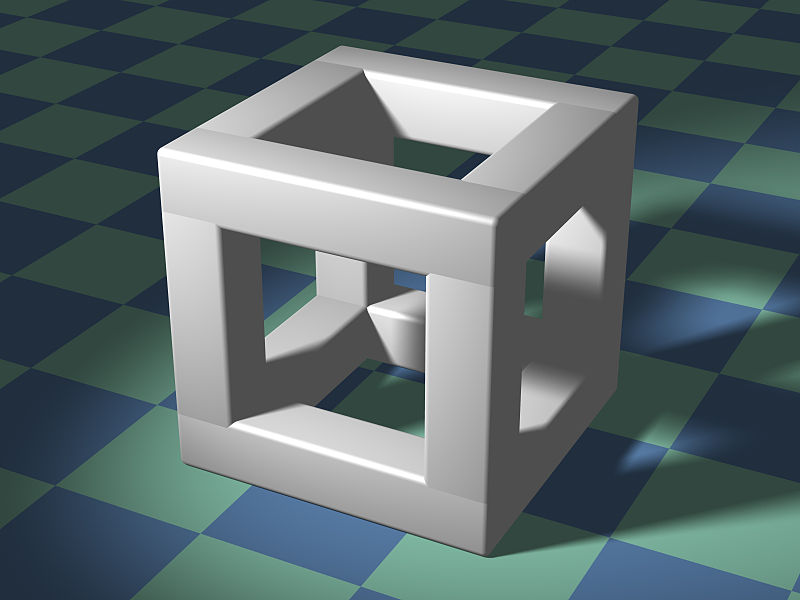
\includegraphics[width=5.5cm]{depth_interp/misc/800px-Cubic_Structure.jpg}}
\end{minipage}
\hfill
\begin{minipage}[b]{0.45\linewidth}
  \centering
  \centerline{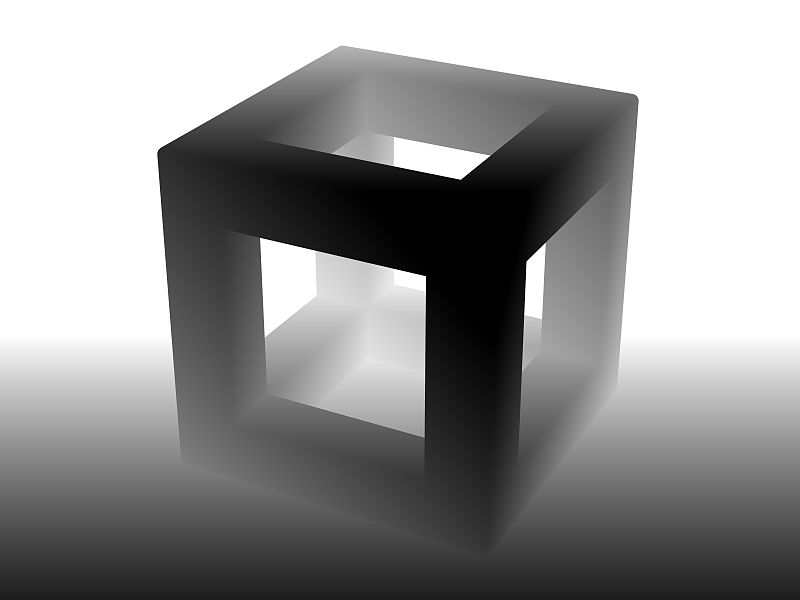
\includegraphics[width=5.5cm]{depth_interp/misc/800px-Cubic_Frame_Stucture_and_Floor_Depth_Map.jpg}}
\end{minipage}
\vfill
\caption{ Left:cubic structure, right: depth map(nearer is darker).}
\label{fig1:def_rgbd}
\end{figure}

\begin{figure}[htb]
\begin{minipage}[b]{0.95\linewidth}
  \centering
  \centerline{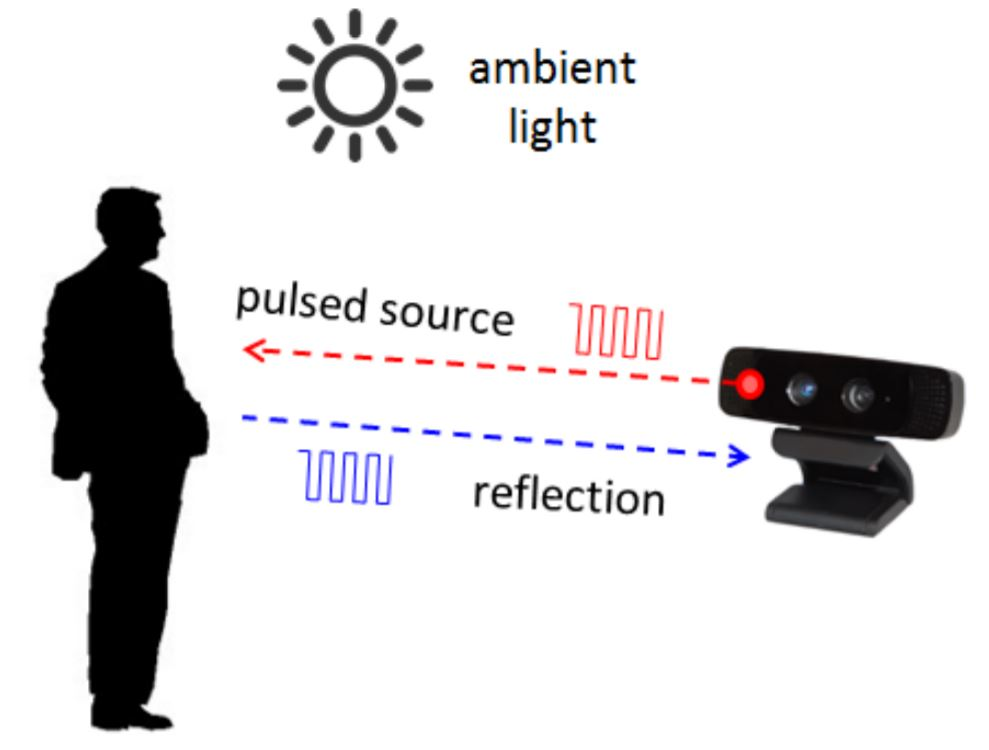
\includegraphics[width=8cm]{depth_interp/misc/tof_camera.JPG}}
\end{minipage}
\vfill
\begin{minipage}[b]{0.95\linewidth}
  \centering
  \centerline{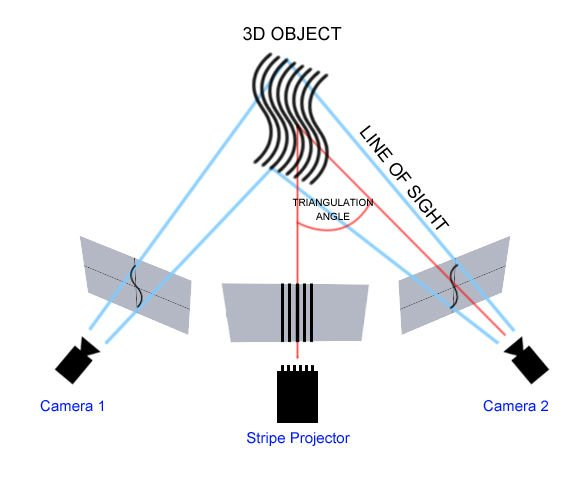
\includegraphics[width=8cm]{depth_interp/misc/structure_light.jpg}}
\end{minipage}
\vfill
\caption{Top: Time-of-Flight camera: low resolution; bottom: Structured light: missing points by occlusion.}
\label{fig1:camera}
\end{figure}
%\begin{figure}[htb]
%\begin{minipage}[b]{0.4\linewidth}
%  \centering
%  \centerline{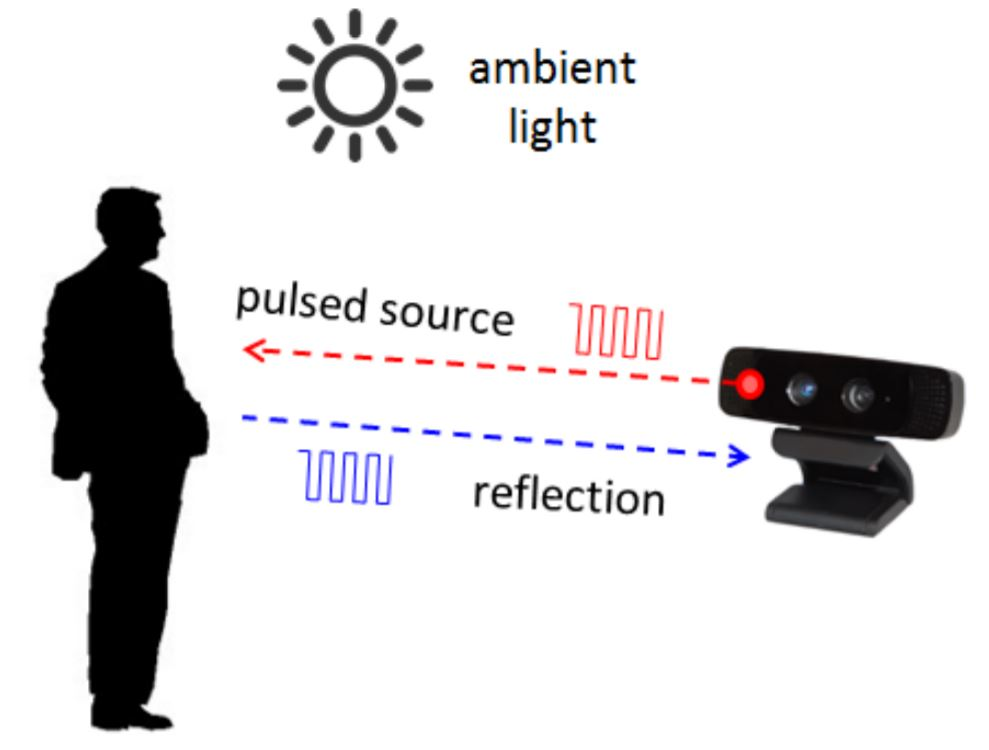
\includegraphics[width=5cm]{depth_interp/misc/tof_camera.JPG}}
%\end{minipage}
%\hfill
%\begin{minipage}[b]{0.5\linewidth}
%  \centering
%  \centerline{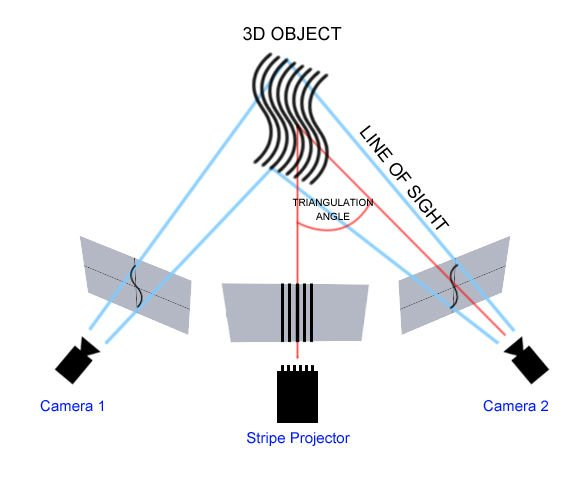
\includegraphics[width=5.5cm]{depth_interp/misc/structure_light.jpg}}
%\end{minipage}
%\vfill
%\label{fig:1.1.camera}
%\caption{Left: Time-of-Flight camera: low resolution; right: Structured light: missing points by occlusion.}
%\end{figure}

\begin{figure}
\begin{minipage}[b]{0.95\linewidth}
\centering
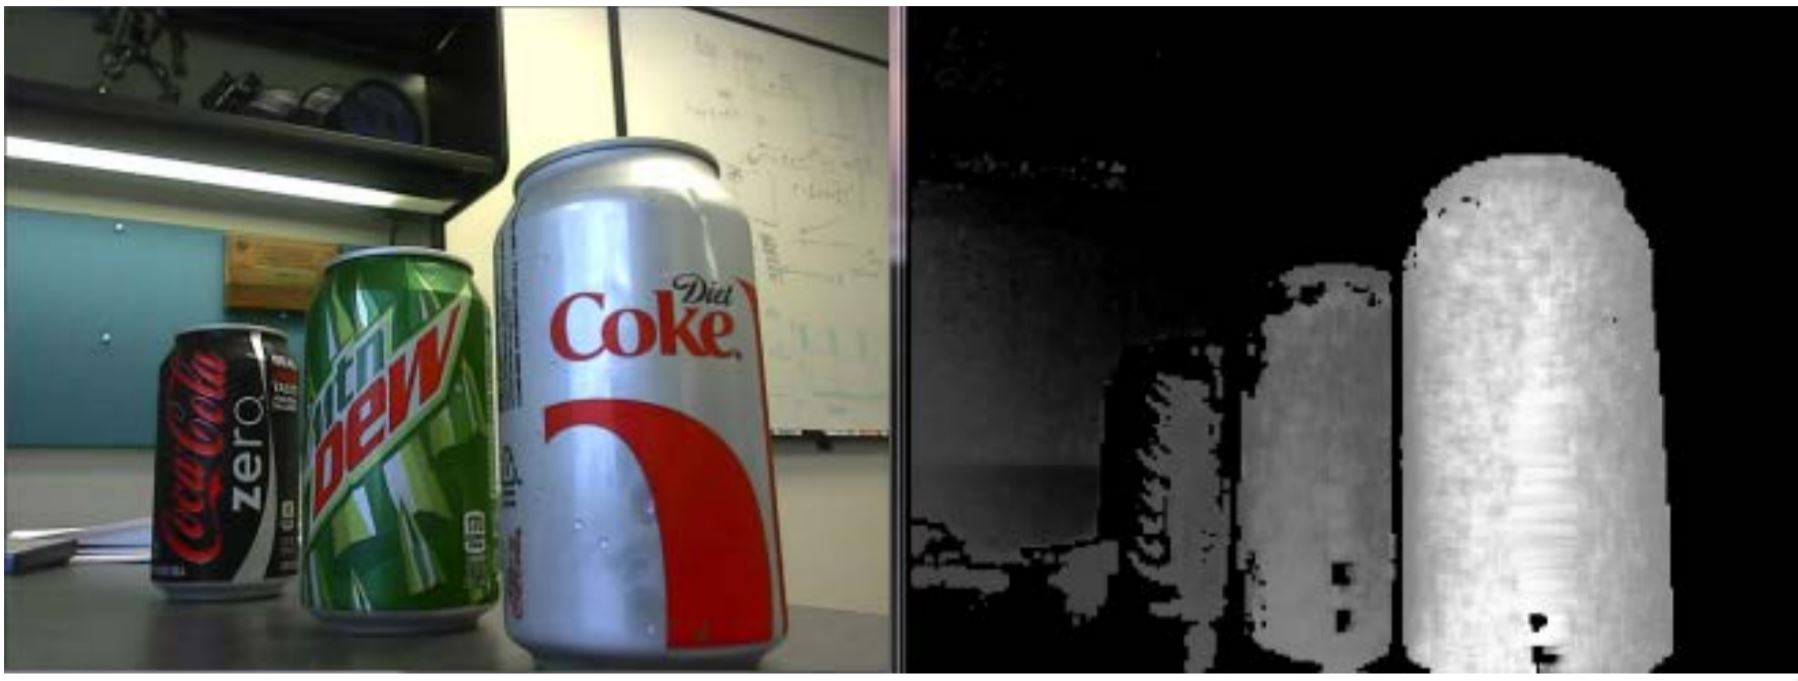
\includegraphics[width = 12cm]{depth_interp/misc/lr_hr.JPG}
\end{minipage}
\vfill
\vspace{0.1in}
\begin{minipage}[b]{0.95\linewidth}
\centering
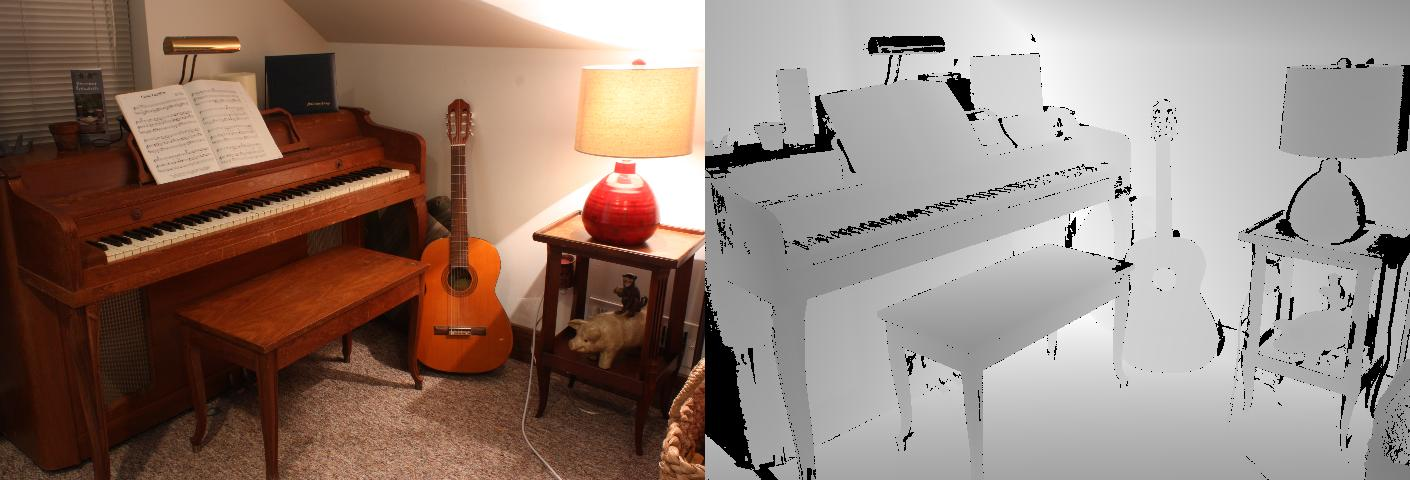
\includegraphics[width = 12cm]{depth_interp/misc/hole.jpg}
\end{minipage}
\caption{Example depth maps.Top: resolution difference; bottom: Missing points. }
\label{fig1:examp_img}
\end{figure}

\section{Background on haze and dehazing}
\label{sec:1.2.dehaze}
Haze and fog are common atmospheric phenomena, caused by the high density and various size of water droplets or particles distributed in the air. Both human vision and images taken under such condition are limited in hazy weather, on the clarity of the contour and the blurred color of objects, especially when the objects are far away or the haze is dense. Figure~\ref{fig1:haze} is an example for the same scene in hazy weather and clear weather: the color in hazy part is generally more "gray" than the normal part, and the edges of different objects are more difficult to tell. This degradation may results in significant problems in many areas, for example when driving in hazy days, the velocity must be slower than clear days to keep safe. Due to the similarity in physical model, under water vision also has the analogous effects. This problem introduces a new task for image processing, namely {\em image dehazing}, or eliminating the haze in images. Another reason driven this study on dehazing algorithms is that air and haze caused by air pollution has attract more and more attentions all over the world, especially in China. We hope the study can do some help in alleviating this problem. 

There are many dehazing algorithms being proposed by now, either based on certain assumptions or other machine learning frameworks. However, there are no general criteria for evaluating the performances of different algorithms. And for existing datasets, most of them are indoor scenes which is not the typical application situation for dehazing algorithms. To build a synthesized hazy scene involves both color images and depth informations, which is a suitable application for RGB-D images. Thus we want to construct a dataset for image dehazing problem, providing outdoor scenes of different weather conditions and ground truth. 

\begin{figure}[htb]
\begin{minipage}[b]{0.95\linewidth}
  \centering
  \centerline{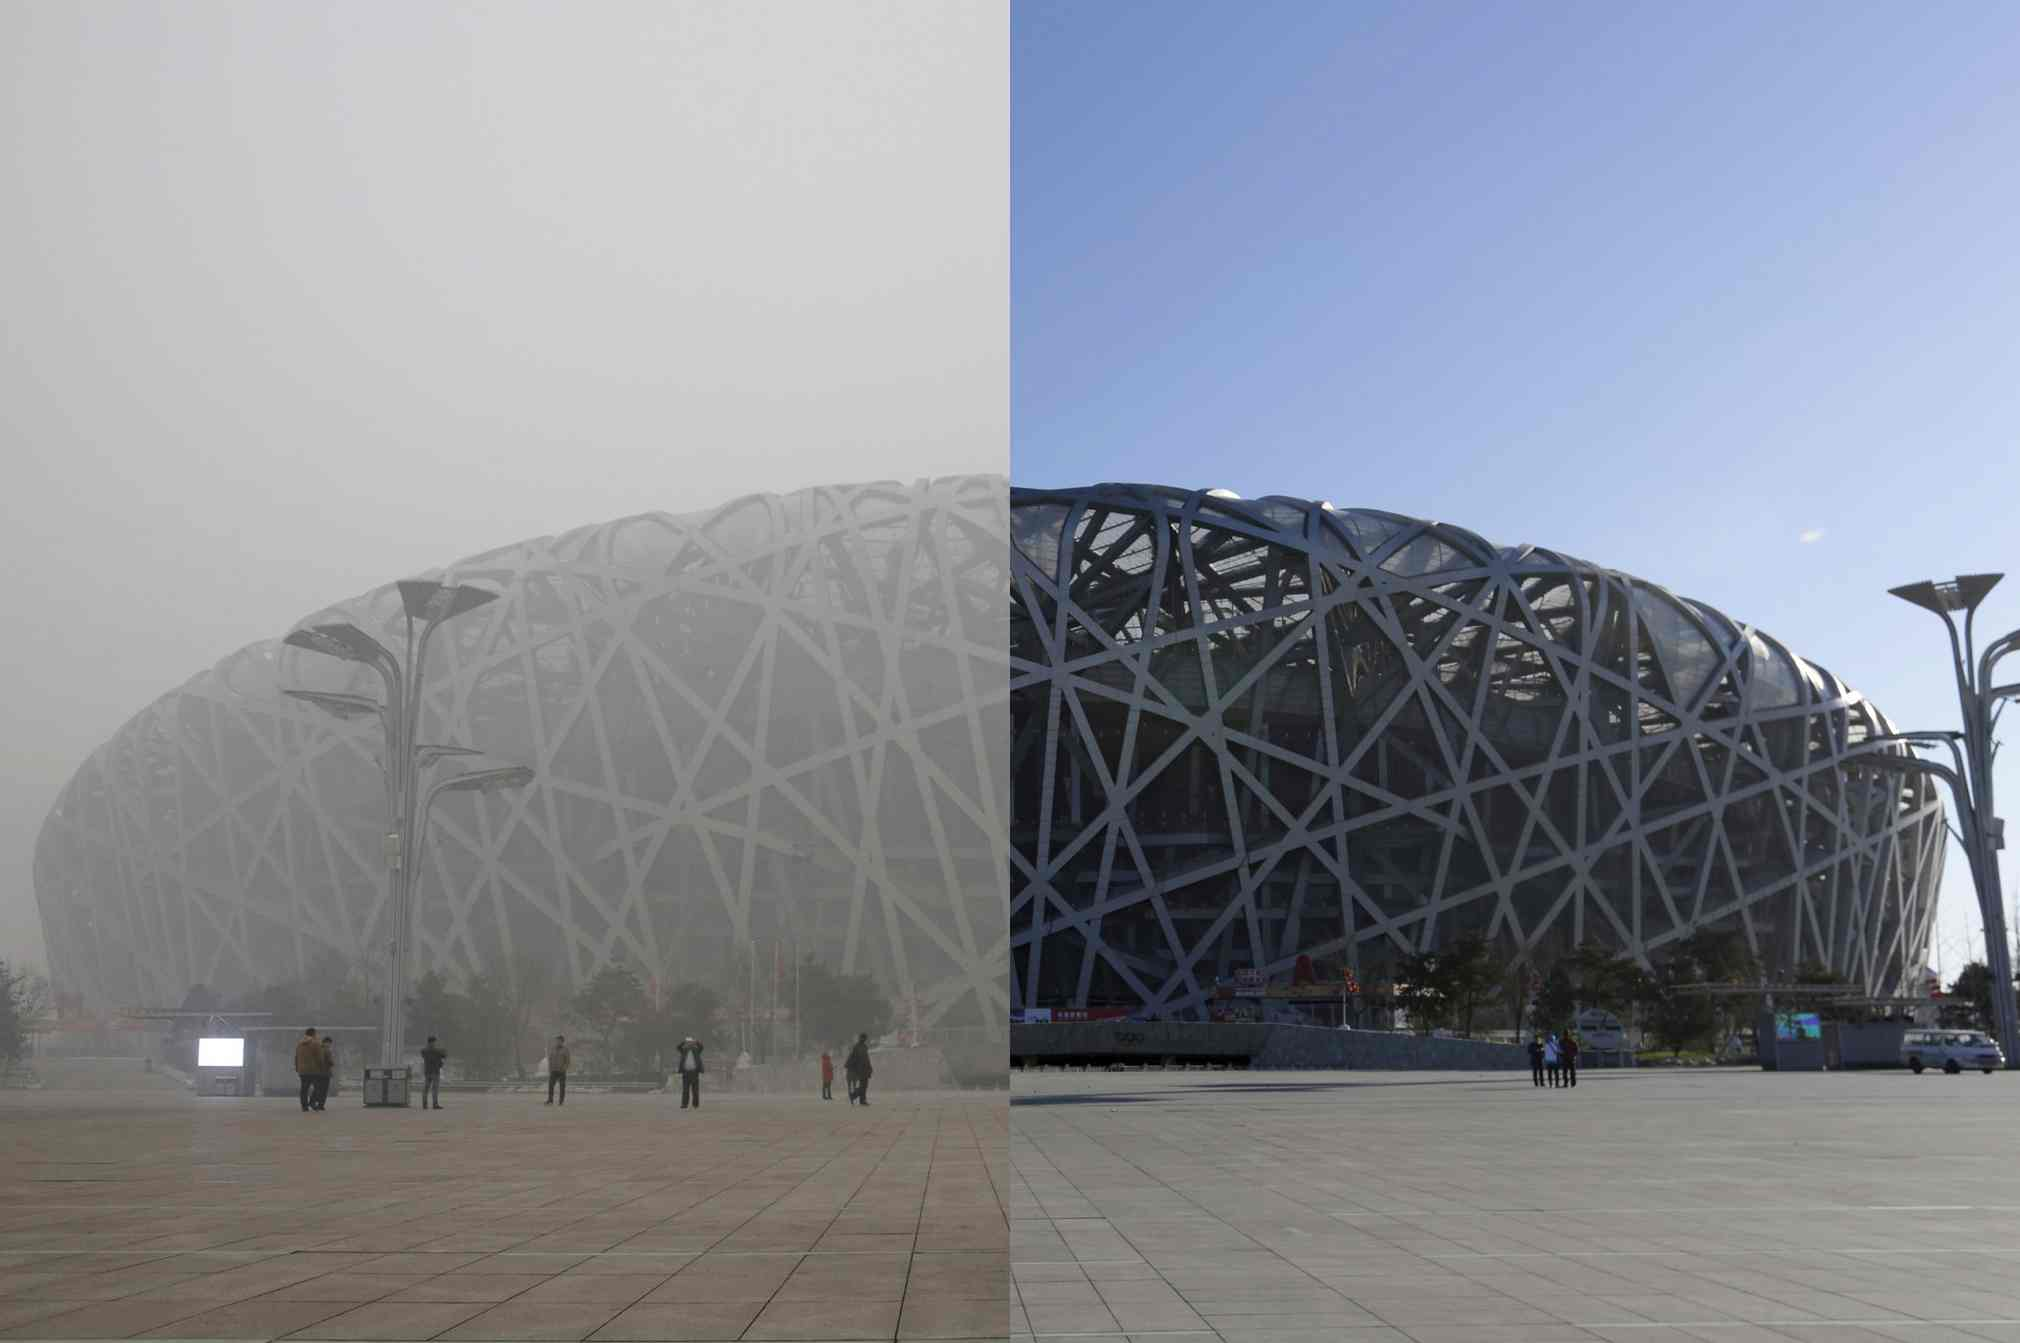
\includegraphics[width = 12cm]{intro/hazeba.jpg}}
\end{minipage}
\caption{The same scene in different weather: left: in hazy weather; right: in clear weather. }
\label{fig1:haze}
\end{figure}


\section{Contribution and future work}
\label{sec:1.3.conclusion}
This thesis has two main contributions. First, an accurate depth map upsampling algorithm is proposed. This method is based on local linear fitting and utilizes the color information to improve the edge quality. We also propose a memory saving implementation to solve the optimization problem. Second, we use RGB-D images to construct an outdoor scene dataset, \emph{HazeRD}, and benchmarked some state-of-the-art dehazing algorithms. Compared to existing dataset, HazeRD provides high-resolution outdoor scenes of different haze levels with ground truth, instead of indoor scenes, which is the typical conditions for the application of dehazing algorithm. 

The work in this thesis also has some limitations. The proposed depth upsampling algorithm is extremely time consuming compared to naive methods such as bilinear or bicubic interpolation. In future work, one direction is to use parallel techniques to accelerate the computing. Besides, the benchmarking results of state of art dehazing algorithms indicates that the main bottleneck lies in the consistency of the estimated transmission of the same objects. In future work, new dehazing algorithms combining image segmentation algorithms should be considered. 


%%%%%%%%%% APPENDIX %%%%%%%%%%

% Redefine sectioning as letters
\setcounter{section}{0}
\let\oldthesection\thesection
\renewcommand{\thesection}{\thechapter.\Alph{section}}
\section{Appendix to Chapter~\ref{cha:has-app}}

Sometimes you might want a chapter-specific appendix numbered separately from
the section numbers in the main text.
This is especially useful when you are dealing with numbered equations or
theorems, and want a way to denote that a result lives in the appendix.
See the source code for this chapter for how this is done.

% Go back to the old section numbering for future chapters
\let\thesection\oldthesection

%%% Local Variables: 
%%% mode: latex
%%% TeX-master: "dissertation"
%%% End: 
